\documentclass[a4paper]{report}

%====================== PACKAGES ======================

\usepackage[french]{babel}
\usepackage[utf8x]{inputenc}

%pour gérer les positionnement d'images
\usepackage{float}
\usepackage{amsmath}
\usepackage{graphicx}
\usepackage[colorinlistoftodos]{todonotes}
\usepackage{url}

%pour les informations sur un document compilé en PDF et les liens externes / internes
\usepackage[hidelinks]{hyperref}

%pour la mise en page des tableaux
\usepackage{array}
\usepackage{tabularx}

%pour utiliser \floatbarrier
%\usepackage{placeins}
%\usepackage{floatrow}
%espacement entre les lignes
\usepackage{setspace}
%modifier la mise en page de l'abstract
\usepackage{abstract}
%police et mise en page (marges) du document
\usepackage[T1]{fontenc}
\usepackage[top=2cm, bottom=2cm, left=2cm, right=2cm]{geometry}
%Pour les galerie d'images
\usepackage{subfig}

%====================== INFORMATION ET REGLES ======================

%rajouter les numérotation pour les \paragraphe et \subparagraphe
\setcounter{secnumdepth}{4}
\setcounter{tocdepth}{4}

\hypersetup{                            % Information sur le document
pdfauthor = {IBRIR Yassine,
            MARTINS MOSCA Jerôme,
            RAHIER Valentine,
            VIOLETTE Paulin},          % Auteurs
pdftitle = {L.I.D.E. -
            Application web pour le developpement},           % Titre du document
pdfsubject = {Rapport de Projet},       % Sujet
pdfkeywords = {},  % Mots-clefs
pdfstartview={FitH}}                    % ajuste la page à la largueur de l'écran
%pdfcreator = {MikTeX},% Logiciel qui a crée le document
%pdfproducer = {}} % Société avec produit le logiciel

%======================== DEBUT DU DOCUMENT ========================

\begin{document}

%régler l'espacement entre les lignes
\newcommand{\HRule}{\rule{\linewidth}{0.5mm}}

%page de garde
\begin{titlepage}
\begin{center}

% Upper part of the page. The '~' is needed because only works if a paragraph has started.

\includegraphics[width=0.35\textwidth]{./img/logo}~\\[1cm]

\textsc{\LARGE M1 Informatique}\\[1.5cm]

\textsc{\Large Concrétisation Disciplinaire}\\[0.5cm]

% Title
\HRule \\[0.4cm]

{\huge \bfseries L.I.D.E.\\
Application Web de Développement \\[0.4cm] }

\HRule \\[1.5cm]

% Author and supervisor
\begin{minipage}{0.4\textwidth}
\begin{flushleft} \large
\emph{Auteurs}\\
Yassine \textsc{Ibrir}\\
Jerôme \textsc{Martins Mosca}\\
Valentine \textsc{Rahier}\\
Paulin \textsc{Violette}\\
\end{flushleft}
\end{minipage}
\begin{minipage}{0.4\textwidth}
\begin{flushright} \large
\emph{Chefs de projet}\\
Alice \textsc{Bazanté}\\
Sullivan \textsc{Chevallier}\\
Pierre-Olivier \textsc{Mainfroid}\\
\emph{Référent:} \\
Laurent \textsc{Garcia}
\end{flushright}
\end{minipage}

\vfill

% Bottom of the page
{\large Octobre - Décembre 2017}

\end{center}
\end{titlepage}


%page blanche
\newpage
~
%ne pas numéroter cette page
\thispagestyle{empty}
\newpage

\renewcommand{\abstractnamefont}{\normalfont\Large\bfseries}
%\renewcommand{\abstracttextfont}{\normalfont\Huge}

\begin{abstract}
\hskip7mm

\begin{spacing}{1.3}

%Résumé

Lorem ipsum dolor sit amet, consectetur adipiscing elit. Sed non risus. Suspendisse lectus tortor, dignissim sit amet, adipiscing nec, ultricies sed, dolor. Cras elementum ultrices diam. Maecenas ligula massa, varius a, semper congue, euismod non, mi. Proin porttitor, orci nec nonummy molestie, enim est eleifend mi, non fermentum diam nisl sit amet erat. Duis semper. Duis arcu massa, scelerisque vitae, consequat in, pretium a, enim. Pellentesque congue. Ut in risus volutpat libero pharetra tempor. Cras vestibulum bibendum augue. Praesent egestas leo in pede. Praesent blandit odio eu enim. Pellentesque sed dui ut augue blandit sodales. Vestibulum ante ipsum primis in faucibus orci luctus et ultrices posuere cubilia Curae; Aliquam nibh. Mauris ac mauris sed pede pellentesque fermentum. Maecenas adipiscing ante non diam sodales hendrerit. Ut velit mauris, egestas sed, gravida nec, ornare ut, mi. Aenean ut orci vel massa suscipit pulvinar. Nulla sollicitudin. Fusce varius, ligula non tempus aliquam, nunc turpis ullamcorper nibh, in tempus sapien eros vitae ligula. Pellentesque rhoncus nunc et augue. Integer id felis. Curabitur aliquet pellentesque diam. Integer quis metus vitae elit lobortis egestas. Lorem ipsum dolor sit amet, consectetuer adipiscing elit. Morbi vel erat non mauris convallis vehicula. Nulla et sapien. Integer tortor tellus, aliquam faucibus, convallis id, congue eu, quam. Mauris ullamcorper felis vitae erat. Proin feugiat, augue non elementum posuere, metus purus iaculis lectus, et tristique ligula justo vitae magna. Aliquam convallis sollicitudin purus. Praesent aliquam, enim at fermentum mollis, ligula massa adipiscing nisl, ac euismod nibh nisl eu lectus. Fusce vulputate sem at sapien. Vivamus leo. Aliquam euismod libero eu enim. Nulla nec felis sed leo placerat imperdiet. Aenean suscipit nulla in justo. Suspendisse cursus rutrum augue. Nulla tincidunt tincidunt mi. Curabitur iaculis, lorem vel rhoncus faucibus, felis magna fermentum augue, et ultricies lacus lorem varius purus. Curabitur eu amet.

\end{spacing}
\end{abstract}

\tableofcontents
\thispagestyle{empty}
\setcounter{page}{0}
%ne pas numéroter le sommaire

\newpage

%espacement entre les lignes d'un tableau
\renewcommand{\arraystretch}{1.5}

%====================== INCLUSION DES PARTIES ======================

~
\thispagestyle{empty}
%recommencer la numérotation des pages à "1"
\setcounter{page}{0}
\newpage

%Ici faire les inputs de toutes les parties

\chapter{Présentation du projet}

\par L'installation de compilateurs peut se montrer compliquée pour les étudiants novices qui suivent les cours d'initiation à la programmation. L'Université d'Angers a donc souhaité simplifier leur apprentissage en centralisant tous les besoins dans un outil de développement en ligne.

\section{Sujet}
%Présentation du sujet : entreprise, encadrement

\par Notre objectif était de réaliser la première version d'un environnement de développement simplifié accessible à partir d'un navigateur web. Il permet d'écrire et de compiler du code rapidement et simplement sans avoir à installer de compilateur sur le poste client (la compilation s'effectuant sur le serveur). Cet outil pourrait être utilisé, dans le cadre des enseignements à l'Université d'Angers, dans plusieurs unités dès la L1 jusqu'à la L3. \\

\par Certaines caractéristiques nous étaient demandées : 

\begin{itemize}

	\item l'édition de code dans un éditeur proposant la coloration syntaxique
	\item la possibilité de compiler le code depuis des compilateurs installés sur le serveur. Le logiciel devra prendre en compte différents langages afin d’être utilisable dans différentes UE
	\item l'accès aux messages d'erreur de la compilation
	\item l'exécution de l'application compilée sur le serveur avec affichage de la sortie
	\item des fonctionnalités avancées devaient être développées telles que l’intégration du débogueur, une gestion plus poussée de l’ensemble de fichiers composant un projet, l'auto-complétion du code, l'intégration d’outils d’analyse

\end{itemize}


\section{Problématique soulevée}

\par L'enjeu principal de ce projet était la sécurité du serveur. En effet, lorsqu'un étudiant tente d'exécuter un programme qui contient des erreurs ou qui demande trop de mémoire CPU, il ne faut pas que le serveur qui gère l'exécution ni les exécutions d'autres étudiants soient ralentis ou bloqués. Pour pallier ces problèmes, nous nous devions d'élaborer une architecture sécurisée afin d'éviter les failles.


\section{Choix des principaux outils et technologies}

\par Lors de la première séance de concrétisation disciplinaire, nos chefs de projet nous ont proposé d'utiliser le framework Symfony pour la réalisation de notre application. Ce framework force à organiser le code et permet une gestion simple de la base de données qui ne dépend pas du type de base de données. De plus, Symfony permet une génération simple des pages grâce à ses controllers et au moteur de template twig.\
Un autre avantage de Symfony est la possibilité d'utiliser des bundles (par exemple, FOSUserBundle permet la gestion des utilisateurs) qui simplifie et accélère véritablement la réalisation des projets. \\

\par Nous avons décidé de placer sous licence libre notre application, c'est pourquoi nous avons choisi MariaDB comme système de gestion de la base de données. De plus, MariaDB a l'avantage d'être légère. \\

\par L'interface graphique a été réalisé grâce au framework Bootstrap qui fournit un thème de base cohérent et esthétique. Bootstrap est simple à utiliser car il se base sur des classes CSS. \\

\par Le choix de la conteneurisation, et plus particulièrement Docker, s'est vite imposé dans l'architecture du serveur. Docker est une méthode de conteneurisation légère qui permet de travailler toujours sur le même environnement (la même image est réutilisée autant de fois que nécessaire) et qui nous a permis d'isoler les compilations et exécutions des programmes.

\section{Répartition des tâches}

\par Afin de travailler efficacement, nous avons séparé le projet en 4 parties autonomes plus ou moins autonomes: Paulin s'est occupé de l'interface graphique, Yassine de l'administration, Jérôme de l'architecture du serveur et Valentine de la communication entre les serveurs.

\subsection{Planning}

Faire le planning
\chapter{Base de données et administration}
\label{ch-bdd-admin}


\section{Conception}

\subsection{Les démarches de conception}

\par Les Acteurs : un acteur représente l’abstraction d’un rôle joué par des entités externes. Dans notre application on distingue principalement deux acteurs qui sont les suivant :

\begin{itemize}
\item L'utilisateur qui peut écrire et compiler son code
\item L'administrateur qui possède les même droits que l'utilisateur mais possède aussi un accès à la page d'administration qui permet de modifier les tables Langages, Détails\_langages et Serveur (voir \ref{ss-partieApp})
\end{itemize}

\subsection{Modèle conceptuel des données (MCD)}
 
\par Le modèle conceptuel des données a pour but de définir de façon formelle la structure de la base de données qui sera utilisée par le système d'information. Il s'agit donc d'une représentation du modèle de données, facilement compréhensible, permettant de décrire le système d'informations à l'aide d'entités. 
La figure suivante présente le modèle conceptuel des données.

\begin{figure}[H]
\centering
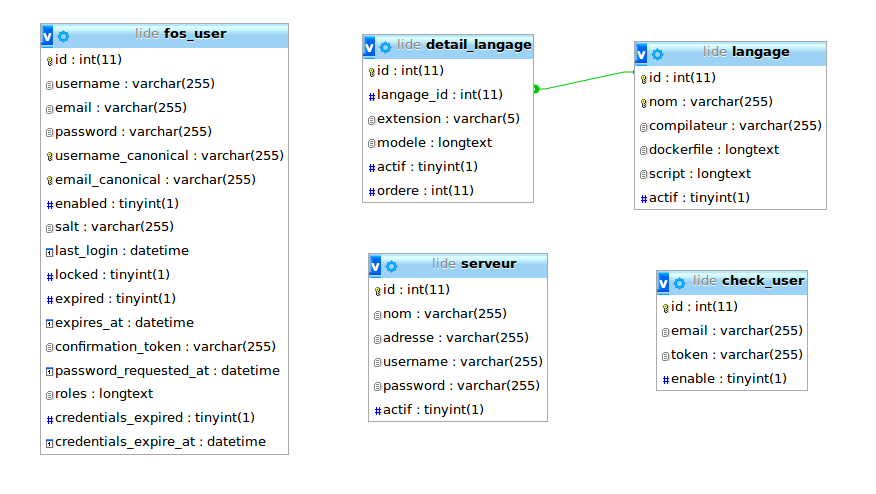
\includegraphics[width=0.8\textwidth]{./img/BDD.png}
\caption{Modèle conceptuel des données}
\end{figure}

\section{Base de données}

\subsection{Partie applicative}\label{ss-partieApp}

\par Les trois tables suivantes contiennent un champ actif qui permet d’activer ou de désactiver le tuple. Par exemple si un serveur est en maintenance ou ne doit pas être utilisé, il pourra être désactivé et réactivé au besoin par l’administrateur. C’est la même chose pour la table langage et details\_langage.


\subsubsection{Serveur}

\par La table Serveur permettra de connaître les serveurs disponibles. S'il y a une surcharge, l’administrateur aura juste à ajouter un nouveau serveur et l’application pourra directement l’utiliser si besoin.

\subsubsection{Langage}

\par Le nom d’un langage est UNIQUE. La table Langage contient le Dockerfile permettant d’installer le nécessaire pour pouvoir compiler/exécuter le langage. Il y a aussi le script qui permet de lancer la compilation avec les fichiers de l’utilisateur ainsi que le compilateur. 
L’avantage de stocker en base de données les langages est de rendre autonome les enseignants. S’ils veulent rajouter un nouveau langage, il leur suffit de l’ajouter avec son Dockerfile et son script.

\subsubsection{Détails langage}

\par La table details\_langage contient les extensions du langage correspondant ainsi qu’un modèle de base (par exemple le Hello World). Cela permet de proposer à l’utilisateur l’extension qu’il veut écrire.

\subsection{Partie administration}

\subsubsection{Fos user}

\par Dans cette table, on sauvegarde tous les informations des utilisateurs.

\subsubsection{Check\_user}

Cette table a pour but de sauvegarder les e-mails des utilisateurs qui n’ont pas encore confirmé leur inscription via le lien de validation reçu dans leur boite mail. 

\section{Administration}

\par Pour mettre en place l’interface administrateur, nous avons utilisé différents outils proposé par Symfony et notamment les bundles FOSUserBundle et EasyAdminBundle.

\subsection{FOSUserBundle}

\par FOSUserBundle est un bundle qui fournit un système de gestion des utilisateurs complet. \\

\par Ce système comprend notamment :

\begin{itemize}
	\item Un formulaire d’inscription avec e-mail de confirmation pour vérifier l'authenticité de l’adresse fournie par l'utilisateur
	\item Un système de récupération de mot de passe (de type <<mot de passe oublié?>>)
	\item Une compatibilité avec la librairie Doctrine pour le stockage en Base de données

\end{itemize}

\par Ces différentes fonctionnalités nous ont permet de sécuriser l’accès à l’application et aussi de paramétrer les droits d’accès à certaines ressources en attribuant des rôles.


\subsection{EasyAdminBundle}

\par Ce bundle nous a permis de créer facilement l’interface administrateur en générant automatiquement les différents formulaires associés aux entités, telles que User et Langage. Il fournit aussi la possibilité d’appliquer les opérations CRUD\footnote{Create, Read, Update, Delete} sur les différentes entités.

\par Doctrine permet de créer des objets (entités) pour gérer les fux entrants et sortants vers la base de données. Ces entités gèrent également le côté relationnel des données. L’ORM Doctrine possède divers commandes permettant la génération automatique des entités. Néanmoins, cette génération reste très basique et il est nécessaire de les modifier afin d’ajouter les relations inter-entités (clé étrangère, relation multidirectionnelle ...) 

\par Les différentes requêtes SQL sont définies sous forme de fonctions dans les fichiers entités, ce qui permet de sécuriser l’appel à ces dernières depuis les contrôleurs.
\chapter{Serveur}

\par Afin de garantir la bonne compréhension des différents termes techniques qui vont suivre, un lexique donnant toutes les définitions nécessaire est disponible en annexe.

\section{Architecture}

\par L’application web vise à être utilisée par des étudiants, certaines conditions de sécurité doivent donc être respectées.
 
\par Les différents programmes doivent pouvoir être lancés sur un environnement vierge indépendant et, bien sûr, isolés du serveur d’exécution afin de prévenir toute corruption de données ou problème de sécurité. Pour répondre à cette problématique, nous nous sommes tournés vers une technique encore jeune et prometteuse : la conteneurisation. Cette technique peut être utilisée via différentes technologies, celle que nous avons choisi est l’une des leader du marché : Docker.

\subsection{Choix effectués}

\subsubsection{Choix de la conteneurisation}


\par La conteneurisation répond à nos critères d’environnement puisqu’elle permet de créer un espace propre indépendant et sans incidence sur l’environnement qui héberge le \gls{service} de chaque exécution. Grâce à cette technique, nous avons pu gérer les problèmes de sécurité et d’allocation de ressources. Nous avons choisi la conteneurisation plutôt que les machines virtuelles car elle a l’avantage d’être plus légère mais aussi plus malléable.  

\subsubsection{Choix de Docker}

\par Docker est une technologie en renouvellement permanent, nous l'avons choisie pour plusieurs raisons. \\

\par D'abord, la conteneurisation avec Docker est une option enseignée par l'Université d'Angers. Aussi, Docker est accessible et documenté. La communauté de ce dernier est très importante. Cela nous donne l’avantage de compléter nos cours en trouvant des solutions à des problèmes réguliers sur des forums, tutoriels et autres outils communautaires.


\subsection{Détails de l'architecture}

\par L’architecture du site se fait en plusieurs étapes. L'architecture actuelle est une première version qui doit être améliorée par une étude de produit plus poussée pour obtenir une architecture définitive.

\subsubsection{Architecture actuelle du site}

\par La version actuelle du site utilise deux serveurs : un serveur pour l’hébergement du site et un autre pour l’exécution des différents programmes créés par les étudiants. Docker permet de créer des conteneurs éphémères sans persistance de données à partir d’une image officielle (présente dans le catalogue de docker) ou d’une image personnelle générée à partir d’un Dockerfile. Quotidiennement, les Dockerfiles sont envoyés au serveur et les images générées afin de s’assurer de la bonne version de ces dernières. Chaque langage utilisé par les étudiants possède une image unique qui lui est propre, de cette façon les images sont plus légères, plus rapides à la génération et ne possèdent que les paquets et applications nécessaires au bon fonctionnement du langage utilisé. 

\par Pour la première version du site, la communication entre l’application web et le serveur d'exécution s’effectue par SSH. Cette connexion permet l'envoi des instructions d'exécution du conteneur ainsi que les directives pour récupérer le fichier généré par l’application web qui sera à compiler. De cette manière, la gestion et la création des conteneurs est dynamique.

\subsubsection{Architecture envisagée}

\par Le client a exprimé le besoin d'utiliser plusieurs serveurs répartis sur tout le territoire français pour les exécutions des programmes. Ces serveurs seront dotés d'un système de load-balancing pour répartir les charges.
La nouvelle architecture a été pensée afin de répondre à cette nécessité et pour assurer une haute disponibilité et respecter la bonne utilisation des principes de Docker.

\par Dans sa version finale, l’application n’aura plus besoin d’un serveur d’hébergement. En effet, l’application entière sera conteneurisée sous forme de services : un service global pour l’exécution des conteneurs, un pour la partie web et un autre pour la base de données.

\paragraph{Avantages de l'architecture envisagée}

\par L’application sera accessible en haute disponibilité. Par conséquent, les différents services pourront posséder un certain nombre de répliques et pourront gérer le load-balancing. Docker s'occupera de la synchronisation des différentes répliques de façon automatique. De plus, si l’une des répliques n’est plus actives, une autre est automatiquement créée empêchant ainsi l'application d'être impactée si un serveur vient à tomber. 

\par La transformation de l’application sous forme de service permet également de créer un Composerfile. Ce fichier permet de lancer les différents services de l’application simultanément mais également de les paramétrer. Ainsi, nous avons la certitude que tous les services sont lancés et ont la bonne configuration et, également, de garder une trace des versions.

\par De plus, un essaim Docker va être mis en place. Tous les serveurs utilisés par l’application feront partie de l’essaim, cela permettra de lier les serveurs entre eux afin de mettre en place le load-balancing.

\\

\par La mise en place d’une telle structure soulève plusieurs questions.

\paragraph{Quelle est la configuration des différents serveurs ?} 

\par Docker est une technologie dite portable mais comme évoqué précédemment cette technologie est encore jeune et possède nombre de limites pour le moment. Pour assurer un fonctionnement identique et sans problèmes des images entre plusieurs serveurs, il faut que ces dernières aient la même configuration (même version de docker, même kernel, et même configuration système que docker pourrait exploiter, comme la prise en charge de la mémoire swap). 

\paragraph{Comment gérer la communication des conteneurs entre les différents serveurs sur des réseaux différents ?} 

\par Docker gère les répliques de services, le reverse proxy ainsi que les différents services SSH. Cependant, si les serveurs ne sont pas sur le même réseau, la communication peut vite devenir problématique. Comment assurer la sécurité ? Comment prioriser le serveur le plus proche physiquement afin de limiter la communication et avoir une vitesse maximale ? Faut-il mettre en place un serveur de communication entre les services au travers des serveurs de l’essaim ? Le principe de communication vers un conteneur à travers un service sur un essaim avec Docker reste encore assez flou à l’heure actuelle. 

\paragraph{Quel service utiliser pour mettre en place l’essaim et le load-balancing ?}

\par Actuellement, deux alternatives dominent le marché : Kubernetes et Docker swarm. Nous avons tenté de mettre en place Docker swarm mais plusieurs problèmes sont apparus. \\

\par Deux façons de faire sont possibles; soit ajouter les serveurs directement à l’essaim soit créer des \gls{dockermachine}s sur les serveurs que l’on ajoute ensuite. Les machines Docker permettent de créer un sous réseau par hôte et d’améliorer la sécurité. Une fois les services définis et l’essaim en place, nous nous sommes rendus compte que la communication entre les services n’était pas aussi aisée que ce que l’on pouvait penser. 

\par Après avoir parcouru la documentation de docker au sujet des essaims, nous nous sommes aperçus que la communication inter-services via l’\gls{essaim} était peu répandue et assez complexe. La mise en place d’un réseau de communication via Consul a été testée mais le temps restant ne nous a pas permis d’aller au bout de cet essai ni de l’étudier en profondeur. Ces différents problèmes ont remis en question l’utilisation de Docker swarm. Une étude des capacités de Docker swarm et de Kurbernetes est nécessaire afin de déterminer laquelle est la plus à même de répondre à nos besoins.

\paragraph{Les avantages de cette architecture}

\par L'architecture envisagée permet de définir notre application en micro services avec une charge répartie sur plusieurs serveurs. Cela permet de rajouter des ressources au besoin. 
\par Elle permet aussi d’avoir une application en haute disponibilité : la gestion des micro services permet, en cas de problème sur l’un des micro services, de minimiser l'ampleur de la panne mais permet également la réplique sur les serveurs pour ne pas avoir de coupure si l’un des serveurs n’est plus disponible. 
\par Les conteneurs permettent d’avoir une sécurité supplémentaire à l’aide de sous-réseaux et d’environnements sans impact sur le serveur d’exécution. L’utilisation de micro services avec un orchestrateur de \gls{conteneur}s tel que Kubernetes ou Docker swarm permet la gestion d'une grande partie de la communication et de la sécurité.   

\subsection{Problèmes rencontrés} 

\par Afin de correspondre aux besoins du client mais aussi dans un but d'optimisation de la sécurité et de l'accessibilité, l’architecture initiale du site a dû être divisée en deux étapes : une architecture basique avec la mise en place d’un système de conteneurs et une communication temporaire. L’architecture temporaire a été pensée afin de minimiser les changements lors du passage à l’architecture envisagée. 
\par La communication a également posé des soucis, notamment lors de l’ouverture du socket SHH qui vient créer le container et ne permet pas à l’étudiant d'accéder au serveur mais uniquement au conteneur.

\par Les différentes configurations de sécurité du réseau de l’Université d’Angers ont été très dérangeantes notamment lors de la génération des images grâce au \gls{dockerfile}. L’utilisation des services SSH étant bloquée, il a également été compliqué de mettre en place la connexion SSH de la première version de l’application. 
\section{Communication Serveur/GUI}

\subsection{Présentation}

\par La communication entre le serveur de l'application et les conteneurs repose sur une connexion SSH. L'application se connecte au serveur contenant les dockers afin de communiquer les messages et d'exécuter les commandes qui lui sont donnés.

\par L'utilisation de Symfony a permis l'utilisation de la librairie libssh2 de PHP. Cette librairie permet de gérer facilement une connexion SSH en PHP.

\subsection{Processus de communication}

\par Le processus de communication repose sur un système de questions/réponses. Le client demande des informations et le serveur lui répond.

\begin{figure}[H]
\centering
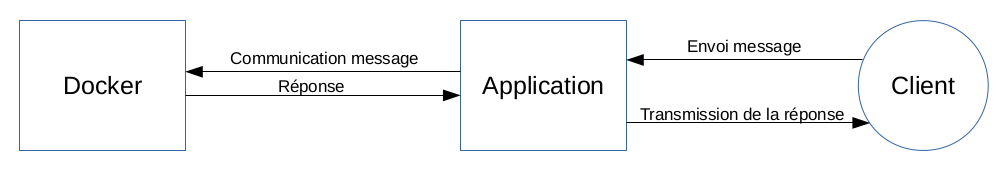
\includegraphics[width=0.8\textwidth]{./img/communication/com.png}
\caption{Schéma simplifié de la communication}
\end{figure}


\subsubsection{Première requête envoyée (clic sur le bouton Lancer)}

\par L'application reçoit la requête du client. Elle va créer la commande qui permet de démarrer un conteneur docker et de lancer le script qui se charge de la compilation et de l'exécution du programme. La commande est ensuite passé au service GestionSSH qui se charge de se connecter en SSH au serveur qui contient les conteneurs et d'exécuter la commande grâce à un shell. 

\par L'application récupère ensuite la sortie standard du programme, toujours grâce au service GestionSSH. Elle répond ensuite au client qui attend toujours la réponse du serveur. Le client affiche ensuite la réponse dans la vue JQConsole.

\subsubsection{Envoi des requêtes suivantes}

\par Dans certains programmes, l'utilisateur a besoin de répondre au programme pour que celui-ci se termine (fonction d'inputs). Dans ce cas, l'application teste si le docker est encore ouvert et le redémarre si oui. Le message est ensuite passé au service de GestionSSH qui se charge de le transmettre au conteneur grâce à SSH.

\par L'application récupère de nouveau la sortie standard du programme pour l'envoyer au client. Cette opération se répète jusqu'à ce que l'exécution du programme soit terminée.

\subsection{Problème de la communication}

\par Le principal problème apparu lors du développement de la communication est dû à la non persistance des objets en PHP. En effet, à la fin de chaque requête, PHP supprime tous les objets qui ont été créés pendant la requête. Il nous était donc impossible de garder une connexion SSH ouverte pendant toute l'exécution du programme. Après de nombreuses recherches, nous avons décidé de créer une nouvelle connexion SSH à chaque nouvelle requête. Le conteneur docker ne se supprimant qu'une fois l'exécution terminée, il était alors possible de communiquer avec lui sans pertes d'informations.

\par L'inconvénient de cette implémentation est que l'application doit récupérer la réponse du docker juste après lui avoir envoyé le message. Pour se faire, le service attend 2 secondes avant de retourner une valeur. Des problèmes apparaissent dès que l'exécution met trop de temps à répondre.

\par Cette implémentation est très critiquable et sera totalement modifiée dans la prochaine version de l'application.
%Paulin VIOLETTE
%Si t'as pas bossé sur l'interface utilisateur t'y touche pas.
%Sauf si la personne dont le nom est écris en haut te dis d'y toucher.
%Deso Paulin moi j'y ai touché
\chapter{Interface Utilisateur}

\section{Présentation}

%Mettre l'image de ma super interface grave stylé
\begin{figure}[h]
  \centering
  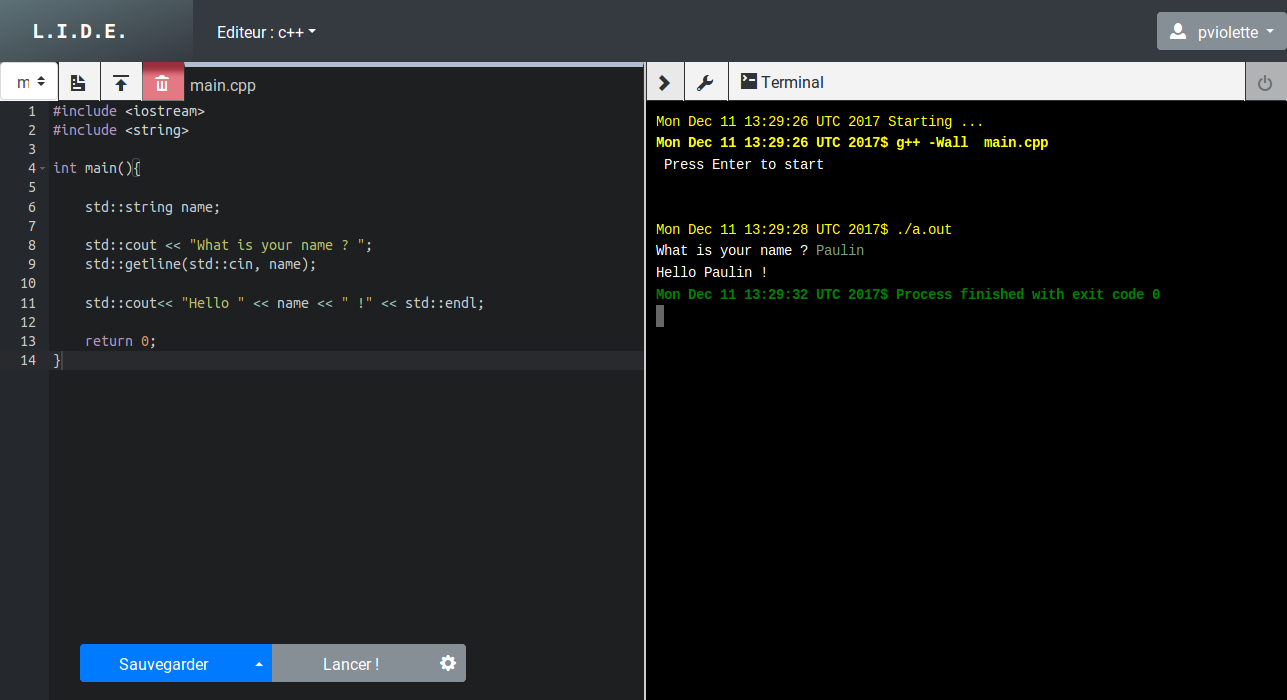
\includegraphics[width=0.8\textwidth]{./img/frontend/example1.png}
  \caption{Interface utilisateur en utilisation}
  \label{}
\end{figure}

Une fois l'utilisateur connecté, il est redirigé vers l'interface de l'application : un éditeur de texte et une console.
L'interface est divisée en quatre parties :
\begin{itemize}
  \item La barre de navigation, contenant les liens vers les autres parties du site (gestion de compte...)
  \item La barre d'outils, qui contient des contrôles spécifiques à l'application
  \item L'éditeur, implémenté par le plugin Ace
  \item La console, implémentée par le plugin jqconsole
\end{itemize}

\section{Outils utilisés}
%Editeur ace
%SweetAlert2 pour les alertes trop swag
%JQConsole vite zef parceque c'est valou qui l'a fait

En plus des outils déjà décrits dans la section \ref{sec-principaux-outils}, l'interface utilisateur utilise plusieurs plugins Javascript.

L'éditeur de texte est Ace\footnote{Voir \url{https://ace.c9.io/}}, un éditeur de texte pour le web supportant la coloration syntaxique de près de 110 langages, mis à disposition sous licence BSD et maintenu comme le principal éditeur pour l'IDE AWS Cloud9. Cet éditeur a pour avantage de supporter de nombreuses fonctionnalités, parmi lesquelles :
\

\begin{itemize}
  \item L'indentation automatique
  \item Chercher/Remplacer avec des expressions régulières
  \item Changement entre tabulation avec des espaces ("soft tab") ou avec une réelle tabulation (caractère \\t, "hard tab").
  \item Numérotage des lignes
  \item Et bien d'autres...
\end{itemize}

Toutes ces raisons nous ont poussés à utiliser ce plugin.

Afin de gérer la console, nous avons choisi d'utiliser le plugin jqconsole (Plus de détails en \ref{subsec-terminal}).

Dernièrement, pour afficher les alertes relatives à l'interface, nous utilisons le plugin SweetAlert2\footnote{Voir \url{https://limonte.github.io/sweetalert2/}} qui nous permet d'avoir des alertes personnalisables et bien plus esthétiques que les alertes classiques.

\subsection{Organisation des templates TWIG}

Le template twig de l'application, \texttt{index.html.twig}, hérite du template \texttt{layout.html.twig}, qui défini une base pour l'application, et qui contient la barre de navigation. Nous avons également créer differents templates pour les modales d'options (de personnalisation, de lancement, d'importation et de création de fichier).

Les templates du bundle FOS (gérant la partie utilisateur du site) sont également redéfini pour s'integrer avec le reste de l'application.

\section{Environnement de Développement}

\subsection{Gestions des langages}
Blabla DB changement de langage

\subsection{Personnalisation}

Toute personne ayant déjà travaillé en groupe sur un projet informatique a pu remarquer que chacun à ses préférences de thème pour un éditeur : certains préfèrent un fond sombre, d'autres un fond clair, etc... L'éditeur Ace est facilement personnalisable et dispose, par défaut, de 24 thèmes. Il était donc assez rapide d'implémenter un formulaire permettant à l'utilisateur de choisir le thème qui lui convient le mieux, lui permettant ainsi de facilement s'approprier son outil de travail.

La police est également personnalisable, permettant à chacun d'utiliser une taille de police qui lui convient.

La console ayant un style implémenté par CSS, il fut de même aisé de créer des thèmes qui s'appliquent grâce à une classe attribuée à l'élément div contenant la console. Pour l'instant, seuls trois styles de console sont implémentés, mais il serait aisé d'en ajouter d'autres dans des versions futures. Chaque style a une classe maîtresse \emph{.console-nom\_style}. On redéfinit ensuite les classes \emph{jqconsole} grâce aux sélecteurs CSS (voir le fichier \emph{console.css}).

Tous ces changements sont pour l'instant uniquement gérés en local (voir fichier \emph{options.js}).

\begin{figure}[!h]
\centering
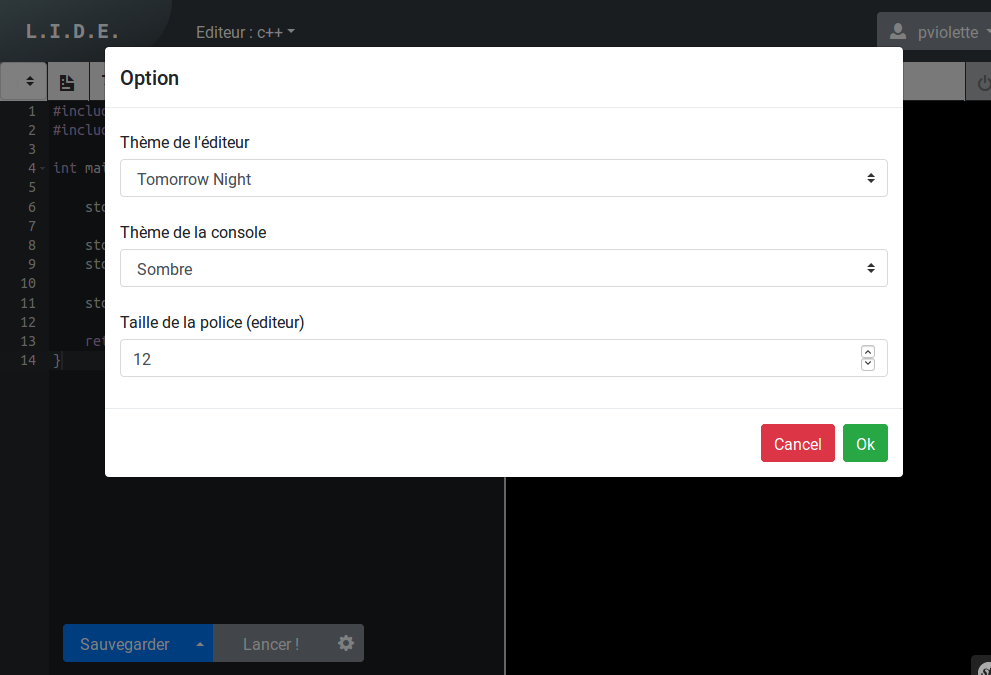
\includegraphics[width=0.8\textwidth]{./img/frontend/example_personnalisation.png}
\caption{Formulaire permettant la personnalisation de l'interface}
\end{figure}

\subsection{Gestions des fichiers}
Tel un véritable EDI, notre application permet la gestion de multiples fichiers. Cette gestion est effectuée sur le navigateur par du javascript.

Les fichiers sont enregistrés dans un prototype contenant deux champs : \emph{name}, le nom du fichier, et \emph{content} son contenu. Ces prototypes sont ensuite stockés dans la variable globale \emph{files}, un tableau de fichier. À chaque changement de fichier en cours d'édition, le contenu de l'éditeur est sauvegardé et est ensuite remplacé par le contenu du nouveau fichier à éditer.

Les fichiers peuvent être créer de deux façons : soit en important un fichier depuis son ordinateur (bouton importation), soit par création à partir de modèles définis par l'administrateur pour le langage.
On laisse également la possibilité de créer des fichiers vides (par exemple pour créer un fichier de données utilisé lors de l'exécution du programme).


\section{Compilation et exécution}

\subsection{Formulaire}

Le formulaire pour compiler et exécuter est généré par Symfony à partir de l'entity \texttt{Execution} et de la classe \texttt{ExecutionType}. Le formulaire comporte 7 champs :
\begin{itemize}
  \item Les paramètres de compilations : arguments passés au compilateurs
  \item Les paramètres de lancement : arguments donnés au programme
  \item Fichiers additionnels : l'utilisateur peut choisir des fichiers depuis son ordinateurs qui seront joints aux fichiers présents dans l'IDE
  \item Une option Compilation Uniquement : si activée, seule la compilation sera effectuée; le programme ne sera pas lancé
  \item{ Un choix de gestion du flux d'entrée :
  \begin{itemize}
    \item Aucun : aucune gestion des entrées n'est effectuée
    \item Interactive : entrée interactive, l'utilisateur écrit sur le flux d'entrée au fur et à mesure de l'exécution du programme.
    \item Texte : les entrées sont définie à l'avance, le programme utilise un fichier comme flux d'entrée.
  \end{itemize}}
  \item Les entrées à donner au programme : seulement si le mode de gestion des entrées Texte est sélectionné.
  \item Un champs caché alimenté par le javascript, contenant le JSON correspondant à la liste des fichiers.
\end{itemize}

\subsection{Lancement de la compilation et de l'exécution}

Le lancement de la compilation et de l'exécution du code écrit est lancé par l'appui sur le bouton "Lancer" qui appelle une fonction JS envoyant une requête AJAX vers la méthode \texttt{ConsoleController::execAction} (fichier ConsoleController.php). Cette requête contient le formulaire qui est ensuite traité : les fichiers vont être écrits dans le système du fichier dans un dossier temporaire, le script de lancement et d'exécution correspondant au langage est récupéré dans la base de données et placé dans ce même répertoire. Une commande, qui va permettre de lancer le docker, est ensuite construite. Cette commande va :
\begin{itemize}
  \item Stopper le container de l'utilisateur s'il existe.
  \item{Lancer un container basé sur l'image correspondante au langage, de nom \emph{id\_[id\_user]A}, paramétré pour être supprimé à la fin de l'exécution de la commande de lancement. Cette commande de lancement va :
  \begin{itemize}
    \item Récupérer le script de lancement sur le serveur de l'application via un wget
    \item Attribuer les droits d'exécution sur ce script
    \item Une commande sed remplaçant les caractères indésirables (dus à la base de données).
    \item Lancer le script avec les bons paramètres
  \end{itemize}}
\end{itemize}

Les paramètres du script à lancer sont :
\begin{itemize}
  \item \texttt{-o 'options\_de\_compilation'}, pour les paramètres à passer au compilateur
  \item \texttt{-f 'fichier1 fichier2...'}, la liste des fichiers de l'utilisateur (récupérée par un wget)
  \item \texttt{-i fichier}, le nom du fichier contenant les inputs s'il est nécessaire
  \item \texttt{-n}, pour un mode non interactif.
  \item \texttt{-a 'agr0 arg1 ...'}, les arguments à donner au programme
  \item \texttt{-c}, pour uniquement effectuer la compilation
  \item \texttt{-w 'wget\_adr'} l'adresse où effectuer le wget.
\end{itemize}

\subsection{Terminal}
\label{subsec-terminal}

\par La mise en place de la console proposait deux options : soit la création d'une vue ad-hoc soit l'intégration d'une vue déjà existante.

\par Notre choix s'est vite tourné vers l'intégration d'une vue déjà existante. La création d'une vue nous aurait certes donné une modularité de la console en ce qui concerne les modifications mais, la console une fois implémentée n'a pas nécessairement besoin de modifications.

\par Après étude de rentabilité, nous avons décidé d'implémenter la vue JQConsole \footnote{https://github.com/replit/jq-console} (utilisée dans repl.it\footnote{\url{https://repl.it/}}, un projet similaire au nôtre) qui correspondait exactement à nos besoins. En plus d'être esthétique, son code source était placé sous licence libre et toutes les fonctions qui nous étaient nécessaires étaient déjà implémentées. L'inconvénient principal est que la modification du code source peut se montrer compliqué, celui-ci étant rédigé en CoffeeScript et étant assez compliqué.

\par Nous n'avions donc plus qu'à intégrer la vue JQConsole à notre interface et faire appel aux bonnes fonctions (notamment JQConsole.Write qui permet d'afficher du texte dans la console et JQConsole.Prompt qui permet de lire du texte) pour obtenir notre console.

\section{Problème rencontré et amélioration possible}

\subsection{Rendre l'interface Responsive}
Un des problèmes de l'interface actuelle est son manque d'adaptabilité sur les plus petits écrans, le design actuel n'ayant pas été conçu dans le but de répondre à cette problématique. Cela est principalement dû au manque d'expérience en web qui nous a mené vers quelque chose de fonctionnel sur ordinateur qui n'est l'est pas sur les plateformes mobiles aux écrans plus petits. C'est une amélioration qu'il serait souhaitable de réaliser dans un version future.

\subsection{Persistance des options de personnalisation et de compilation}

Actuellement, la persistance des options de compilation ou de personnalisation n'est pas assurée. Cette fonctionnalité n'a pas été implémentée principalement par manque de temps mais pourrait rapidement être implémentée en ajoutant les champs nécessaires dans la base de données, afin de lier les préférences à un utilisateur, et en implémentant une méthode renvoyant les choix effectués dans le formulaire de personnalisation au serveur via une requête AJAX, afin que ces choix soit sauvegardés en base de données.

\chapter{Problèmes rencontrés et choix effectués}

\section{Problèmes rencontrés}
\chapter{Conclusion}

\par La réalisation de ce projet a été pour nous tous un exercice très intéressant. Nous nous sommes beaucoup investis et avons tenté de faire au mieux. Le rendu n'est bien sûr pas parfait, mais nous avons appris beaucoup sur le travail d'équipe, la gestion des tâches et le respect du temps.\\
De plus, nous avons pu découvrir de nouveaux outils tels que Symfony, Bootstrap, Docker. \\

\par Notre application est fonctionnelle mais est loin d'être terminée. Il faudrait notamment faire évoluer l'architecture du serveur et de la communication. De plus, il serait intéressant d'ajouter des fonctionnalités comme l'auto-complétion du code, l’intégration du débogueur et l'intégration d’outils d’analyse. \\

\par Nous tenons à remercier nos chefs de projets qui nous ont très bien expliqué le projet et ont su nous guider tout au long de sa conception et de sa réalisation.
\appendix
\chapter{Renseignements sur le repository git}

Lien du repository git :  \url{https://github.com/bazanta/LIDE}
\\Pseudonymes :
\begin{itemize}

	\item Paulin Violette : pviolette-fr
	\item Valentine Rahier : vrahier
	\item Jerome Martins Mosca : ibriryassine
	\item Yassine Ibrir : jejedcll

\end{itemize}

\newpage

%récupérer les citation avec "/footnotemark"
\nocite{*}

%choix du style de la biblio
%\bibliographystyle{plain}
%inclusion de la biblio
%\bibliography{bibliographie.bib}
%voir wiki pour plus d'information sur la syntaxe des entrées d'une bibliographie

\end{document}
